
\begin{figure}[h]
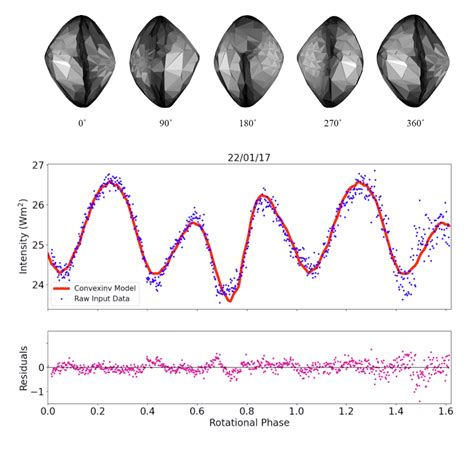
\includegraphics[scale=0.6]{figs/light_curve.png}
\centering
\caption{Ukázka grafu světelné křivky.
Převzato z~\url{https://astrolab.awh.durham.ac.uk/a_lightcurve.html}.}
\label{light_curve}
\end{figure}




\iffalse
rozmer typicky 100 km
1.5\,au daleko (od Země)
1\,au = \,km
úhlová velikost,
$\phi = \arctg{(D/d)}$,
radove $0.1''$

chveni atmosfery (seeing) - odkud je 
vrstvy vzduchu jako male cocky
radove $1''$
adaptivni optika muze korigovat

zakryty hvezd planetkama
hvezda v pozadi
pohyb planetky po obloze
slabsi nez hvezda
pohasnuti hvezdy
zalozeno na presnem mereni casu
secny
vicero pozorovatelu

databáze DAMIT
%\ur{https://astro.troja.mff.cuni.cz/projects/damit/}
pocet modelu
10751 asteroidu
ruznych typu
C, S, aj.
ruzne chemicke slozeni
uhlikate, silikatove, ...
odpovidajici ruznym meteoritum
uhlikatym chondritum, obycejnym chondritum

povrch asteroidu - prelet sondy - prechod k triangulaci
\fi


\iffalse
navazat tim jak jsou tvary ukladany v damit

pocitace si povrch musi rozkouskovat, tvar co dava nejvetsi smysl - trojuhelnik (vysvetlit)

cim vice trojuhelniku, tim presnejsi

vrcholy
plosky

obrazek site jednoducheho tvaru

asteroidy 3D ->
bod ve trirozmernem prostoru,
kartezske souradnice $x,y,z$
spojnice vrcholu tvori hrany, plosky
mnozina vrcholu
$\vec v_i = (x_i, y_i, z_i)$
mnozina plosek
$f_l = (\vec v_i, \vec v j, \vec v_k)$ 
zkraceny popis jen indexy vrcholu
$f_l = (i, j, k)$

obrazek trojrozomerne site

koule jako dvacetisten

%https://en.wikipedia.org/wiki/Polygon_mesh

%https://en.wikipedia.org/wiki/Delaunay_triangulation
\fi



\iffalse
trojrozmerny trojuhelnik
vrcholy $\vec a$, $\vec b$, $\vec c$

delka strany
obvod
severeny uhel
skalarni soucin
soucet uhlu
plocha
vektorovy soucin
teziste
normala
smerovy kosinus (odchylka normaly a smeru ke Slunci)
smerovy kosinus (odchylka normaly a smeru k pozorovateli)
promitnuta plocha
posunuti
otoceni
\fi


\iffalse
tok od Slunce
$\Phi_\odot$
kolik je u Země $1361\,{\rm W}\,{\rm m}^{-2}$

tok na trojúhelník
$\Phi_{\rm i} = \Phi_\odot \mu_{\rm i}$
mu i sklon paprsku dopadajicich na plochu

intenzita zareni
$I = f \Phi_{\rm i}$

funkce rozptylu $f$

tok z trojúhelníku po rozptylu
$\Phi_{\rm e} = I \mu_{\rm e}$

paprsky prichazeji z jednoho, ale jdou do vsech smeru

kazda z plosek ma svoji miru osviceni 
kazda z plosek je (ci neni) pozorovatelna pozorovatelem

https://sirrah.troja.mff.cuni.cz/~mira/fyzika_malych_teles/skripta/
skrpt
skrptpsswd

% https://github.com/miroslavbroz/xitau/blob/master/lc_polygon/lambert.f90

% https://github.com/miroslavbroz/xitau/blob/master/lc_polygon/lommel.f90

% https://github.com/miroslavbroz/xitau/blob/master/lc_polygon/hapke.f90
\fi


\iffalse

Kdyby měl asteroid tvar tříosého elipsoidu a rotoval kolem své nejkratší osy, tak by se obsah promítnuté plochy rovnal: 

\begin{equation}
S = \pi ab
S' = \pi ac
\end{equation}

Otáčení asteroidu mění polohu všech vrcholů trojúhelníku, jejich normál a hodnotu směrových kosinů ($\Phi_{\rm e}$).

meni se kvuli prurezu - elipsa
otaceni asteroidu
otaceni $A$, $B$, $C$ všech trojúhelníků
normaly
smerove kosiny

zmena směru ke Slunci $\vec s$
smerove kosiny

zmena polohy pozorovatele $\vec o$
smerove kosiny

mensi vliv, skoro zapadly kdyz vrha stin
stineni
kratery

mesic
prechod, zakryt, zatmeni
\fi

% https://github.com/miroslavbroz/xitau/blob/master/lc_polygon/integrate_over_S.inc

